\documentclass{beamer}
\usetheme{Madrid}

\usepackage{amsmath, amssymb, amsthm}
\usepackage{graphicx}
\usepackage{listings}
\usepackage{gensymb}
\usepackage[utf8]{inputenc}
\usepackage{hyperref}
\usepackage{gvv}
\usepackage{gensymb}

\begin{document}

\title{MATGEO: 7-7.2-19}
\author{AI24BTECH11020 - Rishika Kotha$^{}$% <-this % stops a space
}
\frame{\titlepage}

\begin{frame}
\frametitle{Question}
Equation of the circle with centre on the Y axis and passing through the origin and the point (2, 3) is
 \\
\begin{enumerate}
    \item $3x^2+3y^2-13y=0$
    \item $3x^2+3y^2+13x+3=0$
    \item $6x^2+6y^2-13x=0$
    \item $x^2+y^2+13x+3=0$
\end{enumerate} \hfill(MATGEO 7-7.2-19)
\end{frame}


\begin{frame}{allowframebreaks}
\frametitle{Solution: Theory}
        \begin{table}[h!]
    \centering
    \begin{tabular}[12pt]{ |c| c| c|}
    \hline
	parameter & Description & value \\ 
    \hline
	 C & Centre & $\myvec{0\\ 13/6}$\\
    \hline 
	 O & point1 & $\myvec{0\\0}$\\
    \hline
	 P & point2 & $\myvec{2\\3}$\\
    \hline   
	 r & radius & 13/6\\
    \hline
    \end{tabular}

    \label{7-7.2-19}
        \end{table}
\end{frame}

\begin{frame}{allowframebreaks}
\frametitle{Given Data}
From the given information,
\begin{align}
	x_1=\myvec{2\\3}, x_2=\myvec{0\\0},n=\myvec{1\\0},c=0 
\end{align}
\begin{align}
    \myvec{4 & 6 & 1 \\
               0 & 0 & 1 \\
               1 & 0 & 0}
               \myvec{u\\f}=\myvec{-13\\0\\0}
\end{align}
The augmented matrix is expressed as
	\begin{align}
        \myvec{4 & 6 & 1 & \vrule & -13\\
         0 &  0 & 1 & \vrule & 0\\                                                 
         1 &  0 & 0 & \vrule & 0}       
\end{align}
\end{frame}
\begin{frame}{allowframebreaks}
\frametitle{Row Operations}
performing sequences of row operations to transform into Echelon form
\begin{align}
	\underleftrightarrow{R_3 \rightarrow R_1-4R_3}
         \myvec{4 & 6 & 1 & \vrule & -13\\
         0 &  0 & 1 & \vrule & 0\\
         0 &  6 & 1 & \vrule & -13}
         \underleftrightarrow{R_1\rightarrow R_1-R_3}
         \myvec{4 & 0 & 0 & \vrule & 0\\
         0 & 0 & 1 & \vrule & 0\\
         0 & 6 & 1 &\vrule & -13}\\
         \underleftrightarrow{R_2\rightarrow R_2-R_3}
         \myvec{4 & 0 & 0 &\vrule & 0\\
         0 & -6 & 0 & \vrule & 13 \\
         0 & 6 & 1 & \vrule & -13}
         \underleftrightarrow{R_3\rightarrow R_3+R_2}
         \myvec{4 & 0 & 0 &\vrule & 0\\
         0 & -6 & 0 & \vrule & 13 \\
         0 & 0 & 1 & \vrule & 0}\\
         \underleftrightarrow{R_1\rightarrow R_1/4, R_2 \rightarrow R_2/-6}
\myvec{1 & 0 & 0 &\vrule & 0\\
         0 & 1 & 0 & \vrule & -13/6 \\
         0 & 0 & 1 & \vrule & 0} 
\end{align}
\begin{align}
   u=\myvec{0 \\ -13/6},f=0
\end{align}
$\therefore$ the equation of the circle is $3x^2+3y^2-13y=0$.
\end{frame}


\begin{frame}{allowframebreaks}
\frametitle{Graph}
\begin{figure}[ht]
\centering
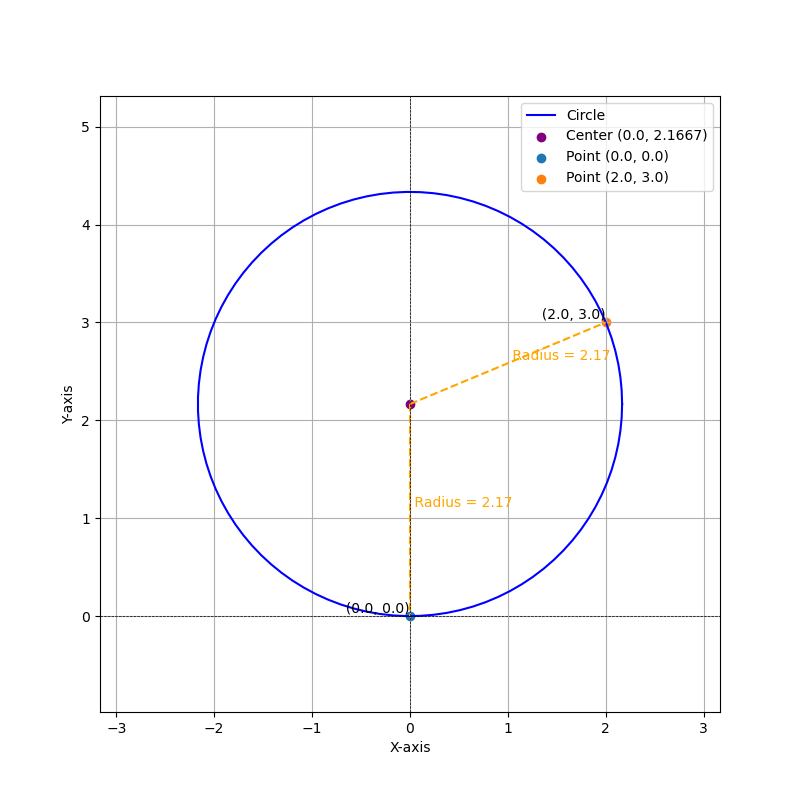
\includegraphics[width=0.7\linewidth]{figs/Fig1.png}
\end{figure}
\end{frame}


\begin{frame}{allowframebreaks}
\frametitle{C-Code}
\begin{figure}[ht]
\centering
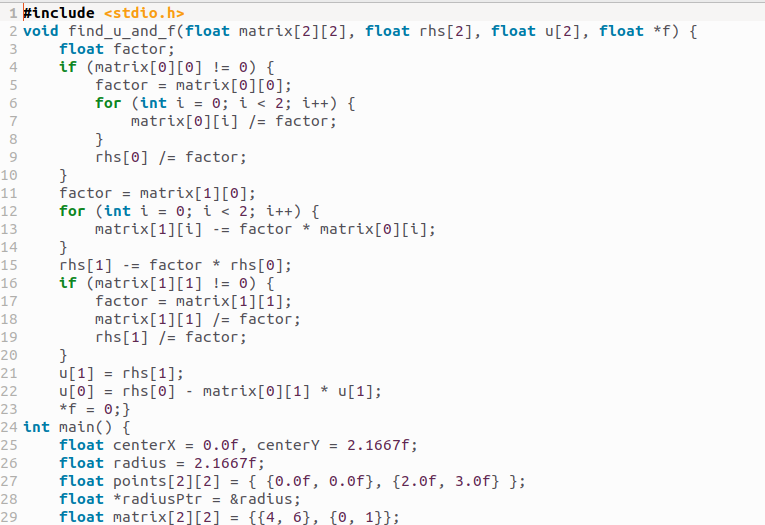
\includegraphics[width=0.7\linewidth]{figs/Fig2.png}
\end{figure}
\end{frame}


\begin{frame}{allowframebreaks}
\frametitle{C-Code}
\begin{figure}[ht]
\centering
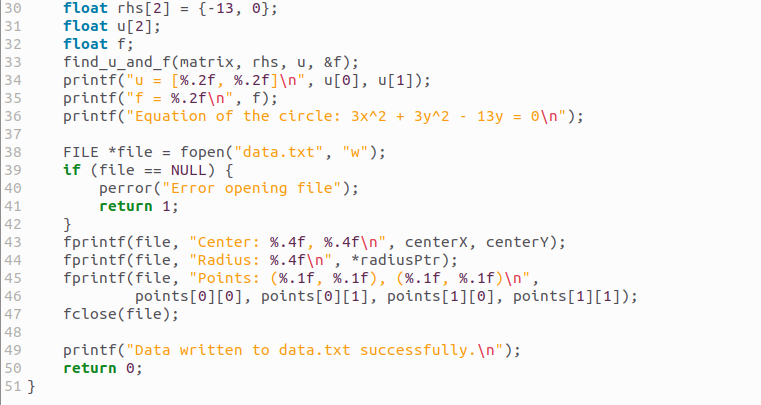
\includegraphics[width=0.7\linewidth]{figs/Fig3.png}        \end{figure}
\end{frame}

\begin{frame}{allowframebreaks}
\frametitle{Python Code}
\begin{figure}[ht]
\centering
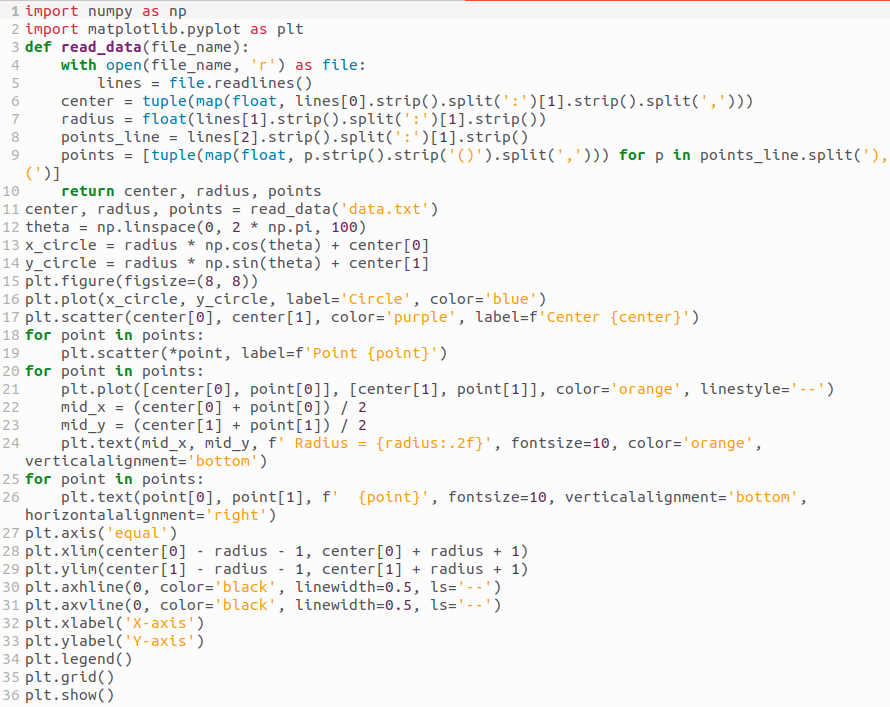
\includegraphics[width=0.7\linewidth]{figs/Fig4.png}
\end{figure}
\end{frame}


\end{document}
